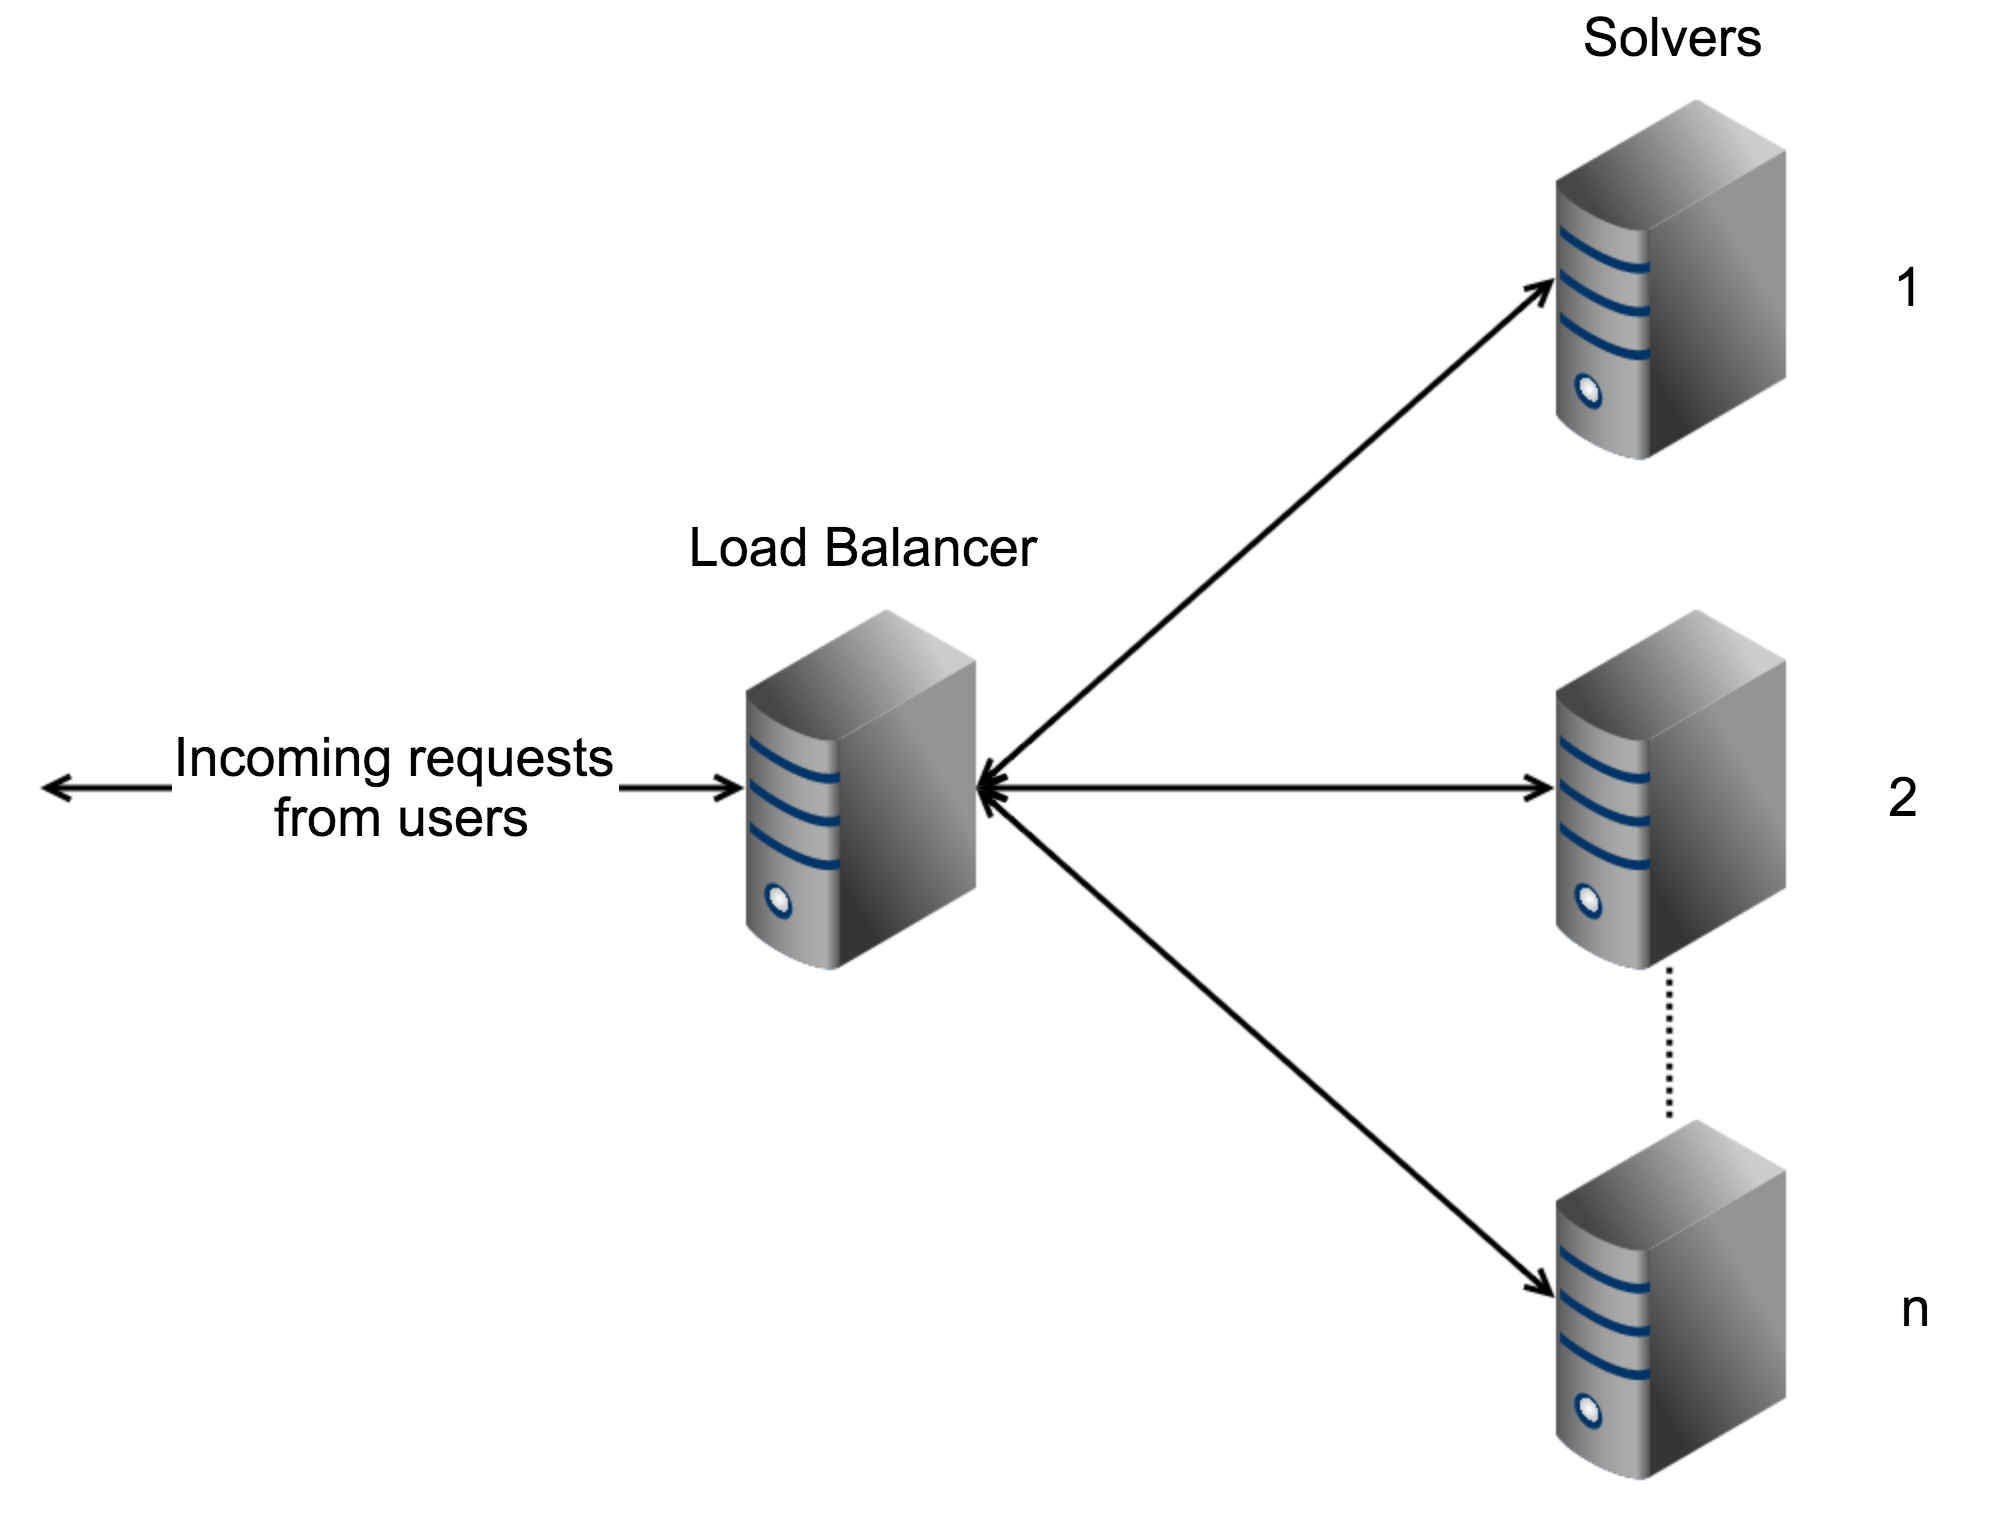
\includegraphics[width=0.5\textwidth]{img/arch}

System Design (recommended size: 1.5 pages)
\begin{enumerate}[(a)]
	\item Resource Management Architecture: describe the design of your system,
		including the inter-operation of the provisioning, allocation, reliability, and monitoring components (which correspond to the homonym features required by the WantCloud CTO).
	\item System Policies: describe the policies your system uses and supports.
		The latter may remain not implemented throughout your coursework, as long as you can explain how they can be supported in the future.
	\item (Optional) Additional System Features: describe each additional feature of your system, one sub-section per feature.
\end{enumerate}

The load balancer has the following interface:
\begin{itemize}
	\item \emph{GET:/solution/<puzzle>} Retrieve a completely filled in Sudoku of <puzzle>.
	\item \emph{GET:/instances} Monitoring, gives a list of all solver machines and their workloads.
	\item \emph{GET:/count} Monitoring, gives a overview of the number of puzzles each solver machine has solved.
\end{itemize}
